\documentclass[tikz,border=10pt]{standalone}
\begin{document}
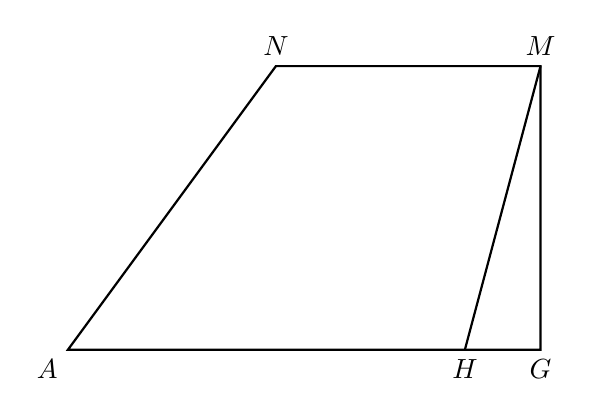
\begin{tikzpicture}[thick, scale=1.2]
    % 1. 定义点坐标
    \coordinate (A) at (-1,0);
    \coordinate (G) at (4,0);
    \coordinate (M) at (4,3);
    \coordinate (N) at (1.2,3);
    \coordinate (H) at (3.2,0);

    % 2. 绘制多边形边框 (ANMG)
    \draw (A) -- (G) -- (M) -- (N) -- cycle;

    % 3. 绘制内部辅助线 (MH)
    \draw (M) -- (H);

    % 4. 标注顶点标签
    \node[below left] at (A) {$A$};
    \node[below] at (G) {$G$};
    \node[above] at (M) {$M$};
    \node[above] at (N) {$N$};
    \node[below] at (H) {$H$};

\end{tikzpicture}
\end{document}